\section{Evaluation}\label{evaluation}

In this section, we evaluate the privacy leakage from attacks.
%In this section, we evaluate the privacy leakage from different attacks.
%The code for all the experiments is made publicly available for easy reproducibility\footnote{Anonymized for Submission}.

\subsection{Membership Inference Attack from Output Predictions {\large(Blackbox setting)}}


The overfitting for GraphSage architecture trained on the three datasets is given in Figure~\ref{fig:NIA}(a).
We evaluate the two blackbox inference attacks exploiting the output predictions from the models: shadow inference which uses auxiliary knowledge on the data distribution and confidence inference which does not use auxiliary knowledge.
Results depicted Figure~\ref{fig:NIA}(b) show that under confidence inference attacks, the inference accuracy is 78.28\% (corresponding to an adversary's advantage of 27.48\%), 63.75\% (an adversary's advantage of 56.56\%), and 60.89\% (an advantage of 21.78\%) for Cora, Citesser, and Pubmed datasets, respectively.
%Results show that under confidence inference attacks, the inference accuracy for Cora is 78.28\% with an adversary's advantage of 27.48\%, 63.75\% inference accuracy for Citesser with an adversary's advantage of 56.56\% and 60.89\% inference accuracy for Pubmed datasets with an advantage of 21.78\%.
In case of shadow model attacks, the inference accuracy for Cora is 62.06\% (representing an adversary advantage of 21.74\%), 60.87\% for Citeseer (an adversary advantage of 24.12\%), 55.51\% for Pubmed dataset (an adversary advantage of 11.02\%).
Membership leakage is thus higher in confidence attack (i.e., without auxiliary knowledge) compared to shadow model attack (i.e., with auxiliary knowledge). While counterintuitive, this result is consistent with similar attack methodology for traditional machine learning models~\cite{princeton}.


\begin{figure}[t]
    \centering
    \begin{minipage}[b]{1\linewidth}
    \centering
    \subfigure[Generalization Error \hspace{0.5in} (b) Inference Advantage]{
    \label{fig:nonmem_soft_label}
    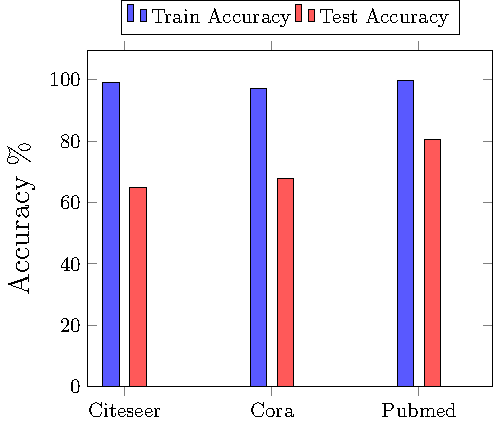
\includegraphics[width=0.5\linewidth,height=3.5cm, keepaspectratio]{figures/BBMIA/GenErr.pdf}
    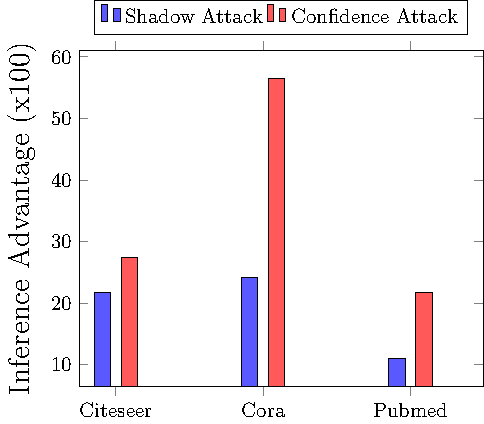
\includegraphics[width=0.5\linewidth,height=3.5cm, keepaspectratio]{figures/BBMIA/NodeIA.pdf}
    }
    \end{minipage}
%\vspace{-2mm}
    \caption{Blackbox membership inference attack uses the output predictions to give adversary an inference advantage.}
    \label{fig:NIA}
%\vspace{-4mm}
\end{figure}



\textbf{Impact of Increasing Number of Layers.} We evaluate the performance of confidence attack on increasing the range of neighbourhood nodes used for aggregating the features (Figure~\ref{fig:numlayers}).
To do that, we extend the range of the message passing algorithm by increasing the number of layers in the GNNs~\cite{klicpera2018combining,Li2018DeeperII}.
On increasing the number of layers from 2 to 6, the inference accuracy decreases by 8\% for GCN. %, GraphSAGE.
Interestingly, the generalization error increases (train accuracy remains the same but the test accuracy decreases) for Cora, Citeseer and Pubmed dataset, but the inference accuracy continues to decrease which indicates that the influence of preferential connections between different nodes in the graph plays a significant role in influencing the inference accuracy. % than the generalization error.
For large number of layers ($>$ 8 layers) in the GNN, for all datasets and architectures, the model completely loses its predictive power.
In general, the inference accuracy as well as prediction accuracy decreases with increasing the range of the message passing algorithm by increasing the layers from 2 to 16.
This implies that the membership privacy leakage is influenced by the structured graph data with preferential connections between different nodes.
Specifically, aggregating features from larger number of nodes results in higher averaging which reduces the distinguishability (over-smoothening of features) as model converges to random walk’s limit distribution~\cite{klicpera2018combining,Li2018DeeperII} which is crucial for inference attacks~\cite{membershipinf,ndss19salem}.


\begin{figure}[!htb]
\centering
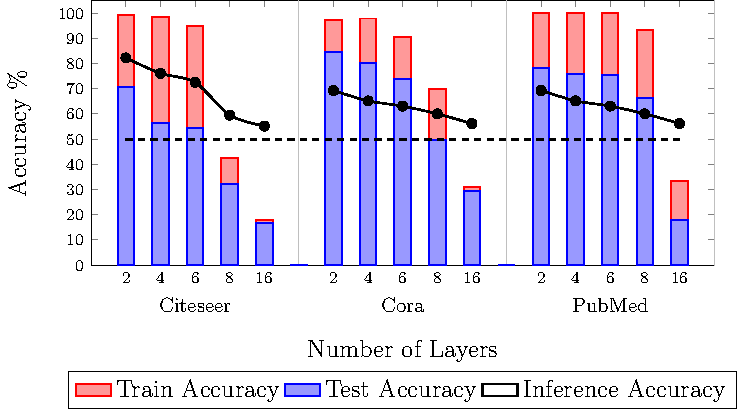
\includegraphics[width=0.4\textwidth,height=3.8cm]{./figures/BBMIA/gsage_numlayers.pdf}
%\vspace{-2mm}
\caption{The inference accuracy and predictive power decreases on increasing the number of layers due to feature oversmoothening from nodes deeper in the graph.}
\label{fig:numlayers}
%\vspace{-2mm}
\end{figure}





\subsection{Membership Inference Attack from Graph Embeddings {\large(Whitebox setting)}}

We exploit the difference in intermediate feature representation of train and test data to perform membership inference attack in a whitebox setting.
Results show that different models trained on PubMed dataset leak significantly more information between 20\% and 36\% over random guess accuracy.
On the other hand, models trained on Citeseer dataset provide to the adversary an advantage between ~7\% and ~17\% over random guess while for Cora dataset it is between 4\% and 7\%.
The embedding is significantly different for train and test data points for PubMed dataset as seen Figure~\ref{fig:whitebox} which result in a higher whitebox membership inference accuracy compared to Cora and Citeseer dataset.
The higher accuracy for Pubmed dataset can be attributed to significant distinguishability of features as seen by visually inspecting in Figure~\ref{embedding}.

\begin{figure}[!htb]
  \begin{center}
    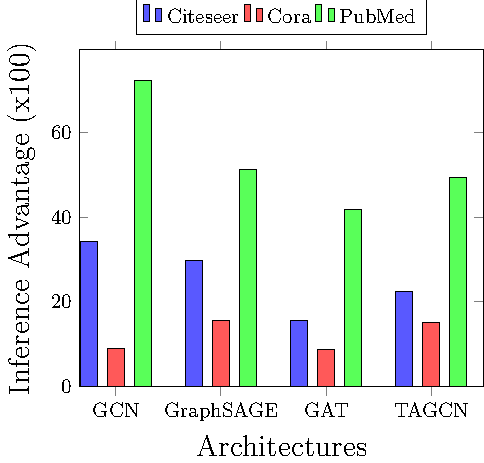
\includegraphics[width=0.65\linewidth]{figures/EmbeddingMIA/whiteboxMIA.pdf}
  \end{center}
  \caption{Adversary advantage for node membership inference from Graph Embeddings.}
  \label{fig:whitebox}
\end{figure}



\noindent The success of the unsupervised whitebox attack is attributed to the message passing which updates the parameters (weights) to specifically ensure higher distinguishability between the data points of different classes for high accuracy on training dataset.
Indeed, the parameters are specifically updated to fit the training dataset resulting in a high distinguishability between feature embedding of train and test data records.
Moreover, the feature embedding for the initial layers are useful since for later layers the features are oversmoothened which also reduces accuracy (as seen in increasing the range of nodes of message passing algorithm).




\subsection{Graph Reconstruction Attack}

The success of graph reconstruction is evaluated on the unseen target graph while the model is trained on the train graph.
The test AUC score for Cora dataset is 0.65 and the average precision is 0.722 while for Citeseer dataset the AUC score is 0.65 and 0.778 average precision.
%In case of 
For Pubmed dataset, we get an average precision of 0.95 on the test set with an ROC of 0.94 in reconstructing the target test graph.
The curve for variation of AUC score and the average precision for the three datasets on the validation sub graph is given in Figure~\ref{fig:valgraphrecon}.

\begin{figure}[!htb]
    \centering
    \begin{minipage}[b]{1\linewidth}
    \centering
    \subfigure[Validation ROC \hspace{1.2in} (b) Average Precision]{
   	\label{fig:mem_soft_label}
    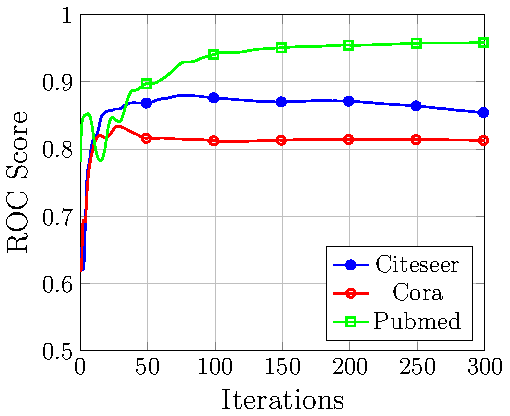
\includegraphics[width=0.5\linewidth]{figures/Reconstruction/roc.pdf}
    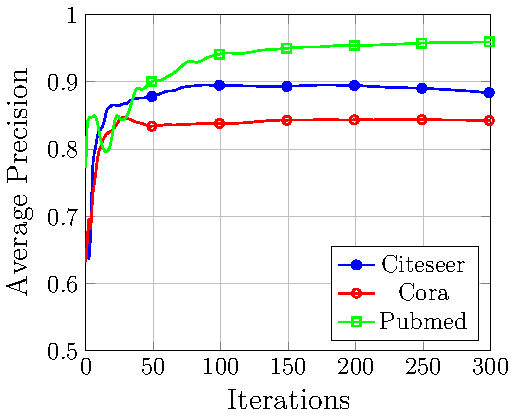
\includegraphics[width=0.5\linewidth]{figures/Reconstruction/ap.pdf}
    }
    \end{minipage}
%\vspace{-3mm}
    \caption{Training curves for AUC score and Average Precision on the validation graph.}
    \label{fig:valgraphrecon}
%\vspace{-1mm}
\end{figure}

\noindent\textbf{Impact of Adversary Knowledge.} On increasing the adversary's knowledge to 50\% of the target graph, we observe an increase the attack performance.
Specifically, the AUC score for Cora increases to 0.76 from 0.65 while the average precision increases to 0.81 from 0.722.
In Citeseer dataset, the AUC score increases to 0.779 from 0.65 while the average precision increases to 0.828 from 0.778.
Finally, for Pubmed dataset showed an increase to 0.95 from 0.94 AUC score and 0.96 from 0.95 average precision.



\subsection{Link Inference Attack}

A direct implication of graph reconstruction attack is inferring whether there exists a link between two nodes in the network by querying the reconstructed adjacency matrix.
This is a binary classification problem.

\begin{figure}[!htb]
  \begin{center}
    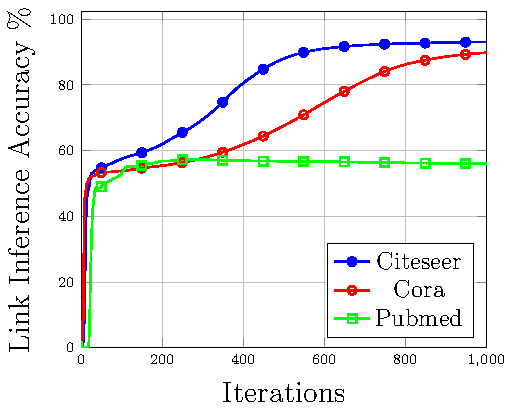
\includegraphics[width=0.65\linewidth]{figures/LinkInfer/LinkInfer.pdf}
  \end{center}
%\vspace{2mm}
  \caption{Link Inference Accuracy Curve over different epochs}
\end{figure}

\noindent For Citeseer dataset, the accuracy of of inference is around 93.39\% while for Cora dataset the inference accuracy is 90.73\% and 57.28\% for Pubmed dataset.
This indicates an adversary advantage of 86.78\% (Citeseer), 81.06\% (Cora) and 14.56\% (Pubmed).
The same train-test-validation distribution is used for the three datasets with 30\% train records and 60\% test records and remaining 10\% as validation records.



\subsection{Attribute Inference Attack}

In case of attribute inference attacks, we evaluate two state of the art embedding models: Node2Vec and DeepWalk, using three attack models: Neural Networks (NN), Random Forest (RF) and Support Vector Machine (SVM).
We generate embeddings using the two algorithms on Facebook and LastFM dataset which contain gender and location as sensitive attributes, respectively.
That is, the adversary infers user gender as a target sensitive attribute in Facebook dataset classified into one of three classes: Male, Female and Others.
The location target attribute for LastFM dataset is categorized in 18 locations for the users in the network.

\begin{figure}[!htb]
    \centering
    \begin{minipage}[b]{1\linewidth}
    \centering
    \subfigure[LastFM \hspace{1.2in} (b) Facebook]{
   	\label{fig:mem_soft_label}
    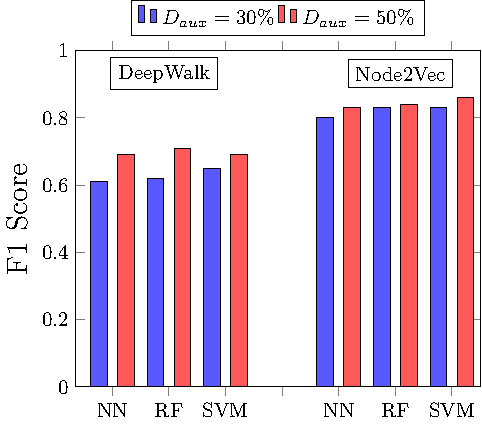
\includegraphics[width=0.5\linewidth,height=3.5cm, keepaspectratio]{./figures/AIA/lfm_AIA.pdf}
    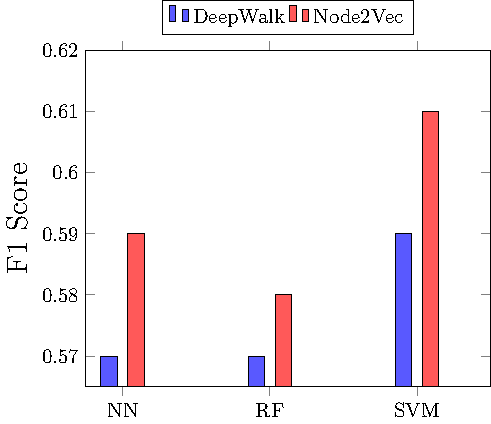
\includegraphics[width=0.5\linewidth,height=3.5cm, keepaspectratio]{./figures/AIA/fb_AIA.pdf}
    }

    \end{minipage}
%\vspace{-3mm}
    \caption{F1 score for different attack classifiers to infer sensitive attributes.}
    \label{fig:aia}
\end{figure}

The inference attack performance is given by the F1 score (Figure~\ref{fig:aia}). %as shown in Figure~\ref{fig:aia}.
For Facebook, the graph embedding using DeepWalk resulted in an F1 score of 0.57 for NN, 0.58 for RF and 0.59 for SVM classifier.
On the other hand, Facebook's Node2Vec embedding showed an F1 score of 0.59, 0.57 and 0.61 respectively for NN, Rf and SVM attack classifier.
In case of LastFM, we found the attack F1 scores for Node2Vec for higher than DeepWalk embeddings.
The F1 score for DeepWalk 0.61, 0.62 and 0.65 corresponding to NN, RF and SVM attack classifier while the F1 score using Node2Vec embeddings are 0.80, 0.83 and 0.83 for NN, RF and SVM.

\textbf{Impact of Adversary's Knowledge.} The performance of the attack model for Facebook dataset did not increase by much.
On increasing the knowledge of the adversary's auxiliary dataset from 30\% to 50\%, the confidence of attack on LastFM dataset increases.
For DeepWalk algorithm, the attack F1 score increases to 0.69 from 0.61 for NN, 0.71 from 0.62 for RF and 0.69 from 0.65 for SVM attack classifier.
On the other hand, for Node2Vec, the attack model F1 score increased to 0.83 from 0.80 for NN, 0.84 from 0.83 for RF and 0.86 from 0.83 for SVM.
